\section{Introduction and Motivation}

Despite extensive use in financial applications to achieve consensus between non-trusting parties \cite{Killeen2015}, blockchains have seen limited deployment in the energy space \cite{DeutscheEnergie-AgenturGmbHdena2016} and have not been considered for coordinating DERs to manage network constraints \cite{Bonneau2015}.

We structure the remainder of the paper as follows: Section \ref{sec:blockchain} provides a brief overview of blockchains and smart contracts. Section \ref{sec:litreview} provides a survey of previous literature on dispatch of DERs in microgrids, decentralized optimization techniques, and blockchain use in energy applications. Section \ref{sec:formulation} presents the formulation of the optimal power flow problem.


\begin{figure}[h]
\resizebox{0.45\textwidth}{!}{
\begin{tikzpicture}[scale=0.2,
bluenode/.style={circle, draw=blue!60, fill=blue!5, very thick, minimum size=7mm},
rednode/.style={circle, draw=red!60, fill=red!5, very thick, minimum size=5mm},
]
%Nodes
\node[bluenode]   (leftend)[text width=1.8cm]   {downstream nodes};
\node[bluenode]  (x)       [right=of leftend] {$f(x),x\in\mathcal{X}$};
\node[rednode]   (z)       [right=of x] {$g(z),z\in\mathcal{Z}$};
\node[bluenode]  (rightend)       [right=of z,text width=1.5cm] {upstream nodes};
 
%Lines
\draw[<->] (leftend.east) -- (x.west);
\draw[<->] (x.east) -- (z.west);
\draw[<->] (z.east) -- (rightend.west);
\end{tikzpicture}}
\caption{Sample problem structure, with arrows showing shared variables.}
\label{fig:nodefigure}
\end{figure}

%%%%%%%%%%%%%%%%%%%%%%%%%%%%%%%%%%%%%%%%%%%%%%%
\section{Blockchains and smart contracts}
\label{sec:blockchain}

\lipsum[4]
\begin{figure} 
\centering
\includegraphics[scale = 0.35]{Blockchain_Graphic.pdf}
\caption{Symbolic representation of the data in a blockchain, showing blocks $B^0$ to $B^{t+1}$ with detail of block $B^t$. Blocks are linked by their cryptographic hashes $\Upsilon(B^t)$, securing the contents from alteration and allowing transparent auditing of system history. Messages $M_i^t$ contain information about changes to the system state, such as energy transfers or payments.}
\label{fig:blockfig}
\end{figure}

The general architecture of blockchains is described in \cite{Wood2014} and illustrated in Fig. \ref{fig:blockfig}. 
\lipsum[21]

%%%%%%%%%%%%%%%%%%%%%%%%%%%%%%%%%%%%%%%%%%%%%%%
\section{Prior Literature}
\label{sec:litreview}

As discussed in \cite{Ton2012}, 
Microgrids are electricity networks may operate in both grid-connected and self-sufficient modes. Surveys of approaches to microgrid management can be found in \cite{AhmadKhan2016,Minchala-Avila2015}. Decentralized algorithms have been explored for coordinating electric vehicles \cite{LeFloch2016,LeFloch2016a}, smart inverters \cite{Sondermeijer2016}, and for fleets of diverse DERs \cite{Mhanna2016,Tsai2015,Wang2016}. 
\lipsum[25]

%%%%%%%%%%%%%%%%%%%%%%%%%%%%%%%%%%%%%%%%%%%%%%%



%%%%%%%%%%%%%%%%%%%%%%%%%%%%%%%%%%%%%%%%%%%%%%%
\section{Optimal Dispatch Formulation}
\label{sec:formulation}

The distribution network is modeled as an undirected radial graph $\mathcal{G}(\mathcal{N},\mathcal{E})$, consisting of a set of nodes $\mathcal{N}$ and a set of distribution lines (a.k.a. edges) $\mathcal{E}$ connecting these nodes. Using the notation described in \cite{Li2015c}, we index the nodes in $\mathcal{N}$ by $i = 0, 1, \dots, n$, where node $0$ represents the root node (substation) and other nodes in $\mathcal{N}$ represent branch nodes. We also denote a line in $\mathcal{E}$ by the pair $(i, j)$ of nodes it connects where $j$ is closer to the feeder $0$. We call $j$ the parent of $i$, denoted by $\pi(i)$, and call $i$ the child of $j$. Denote the child set of j as $\delta(j):=\{i:(i,j)\in \mathcal{E}\}$. Thus a link $(i, j)$ can be denoted as $(i, \pi(i))$. 

\begin{subequations}\label{eqn:distflow}
\begin{align}
p_i &= P_i -\sum_{k\in\delta(i)}P_{k} + \text{r}_{i}l_{i}, \quad i=0,\dots,n \label{eq:pf1}\\
q_i &= Q_i -\sum_{k\in\delta(i)}Q_{k} + \text{x}_{i}l_{i}, \quad i=0,\dots,n \label{eq:pf2}\\
v_i &= v_{\pi(i)}+ 2(\text{r}_{i}P_{i} +\text{x}_{i}Q_{i}) - (\text{r}_{i}^2 + \text{x}_{i}^2)l_{i}, i=1,\dots,n  \label{eq:pf3}\\
l_{i} &= \frac{P_{i}^2 + Q_{i}^2}{v_i}, \quad i=1,\dots,n  \label{eq:noncvxbranchflow}
\end{align}
\end{subequations}
where $S_0=0+\mathbf{i}0$ at the slack bus. Equations in \eqref{eqn:distflow} define a system in the variables $(P,Q,l,v):=(P_i,Q_i,l_i,v_i, \ \forall \ $i$ \ \in \mathcal{N})$, which do not include phase angles of voltages and currents. Given $(P,Q,l,v)$, phase angles can be uniquely determined for radial networks \cite{Farivar2013}.


%%%%%%%%%%%%%%%%%%%%%%%%%%%%%%%%%%%%%%%%%%%%%%%
\section{Blockchains and ADMM}
\label{sec:blockchainadmm}

\lipsum[3]


%%%%% ALGORITHM BLOCK
\RestyleAlgo{boxed}
\begin{algorithm}
 \DontPrintSemicolon
  \SetKwFunction{FMain}{Main}
  \SetKwProg{Fn}{$\mathbf{P_i}$}{:}{}
  \Repeat{$\|r^k\|_2 \leq \epsilon_{pri}, \ \|s^k\|_2 \leq \epsilon_{dual}$}{
  \Fn(\textit{Private Optimization, compute locally}){}{
        Gather private constraints\;
        Compute $\tilde{x}_i$ and send to smart contract $S_1$\;
  }
  \SetKwProg{SOne}{$\mathbf{S_1}$}{:}{}
  \SOne(\textit{Security Smart Contract, on blockchain}){}{
        Check $\tilde{x}_i$ for feasibility\;
        If attack detected, flag node $i$ \& adjust $\tilde{x}_i$\;
        Update $u$\;
        % Not sure if we want to show the condition on only updating after having received all devices' updates.        
        \If{$\|r^k\|_2 \leq \epsilon_{pri}, \ \|s^k\|_2 \leq \epsilon_{dual}$}{
        Compute final schedule and clearing prices\;
        Send schedule to $S_2$
        }
  }
  }
  \SetAlgoCaptionLayout{footnotesize}
  \caption{Computational elements in the microgrid control system. Function $\mathbf{P_i}$ is executed locally by each device participating in the market.} \label{algorithm:eventsequence}
\end{algorithm}

Algorithm \ref{algorithm:eventsequence} \lipsum[5]



%%%%%%%%%%%%%%%%%%%%%%%%%%%%%%%%%%%%%%%%%%%%%%%
\section{Implementation: Test network}
\label{sec:implementation}

Details available at:

\texttt{github.com/emunsing/energyblockchain}


Figure \ref{fig:power} demonstrates that \lipsum[6]

\begin{figure} 
\centering
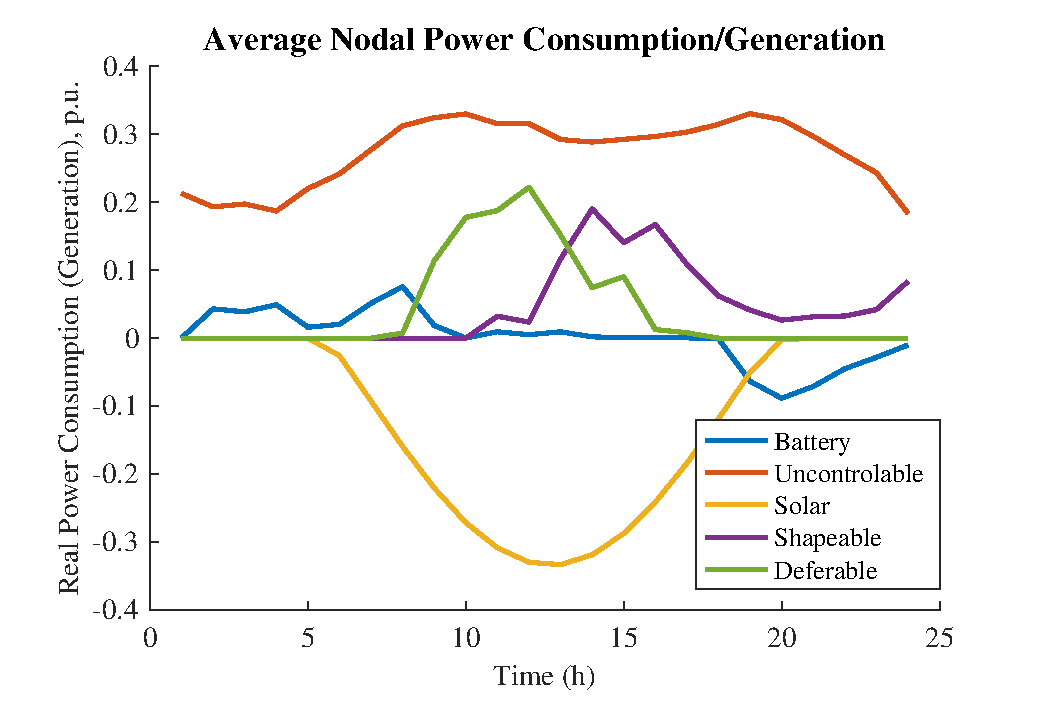
\includegraphics[scale = 0.52]{Power.eps}
\caption{Schedule of commitments generated by the ADMM algorithm and stored to the smart contract.}
\label{fig:power}
\end{figure}

\lipsum[10-11]

%%%%%%%%%%%%%%%%%%%%%%%%%%%%%%%%%%%%%%%%

\section{Conclusions}
\label{sec:conclusions}

\ifarticle \addtolength{\textheight}{-15cm} \fi % This command serves to balance the column lengths on the last page of the document manually. It shortens the textheight of the last page by a suitable amount. This command does not take effect until the next page so it should come on the page before the last. Make sure that you do not shorten the textheight too much.


\lipsum[16-18]